\chapter{Statistical Machine Translation}
\label{chap:SMT}
\section{Motivation behind SMT}
	\textbf{SMT} unlike RBMT doesn't depend on complex rules to translate from source language to target language. Also, rules are written with keeping a pair of language in mind, hence can't be generalized over other pairs. SMT on the other hand relies heavily on availability of parallel corpora. There is no dependency on pair of language involved in translation. 	

\section{Noisy Channel Model of Translation}
SMT is based on simple Noisy channel model. For instance in the case of Foreign (\textit{f}) $\rightarrow$ English (\textit{e}), the posterior probability of most likely English sentence given the foreign sentence can be broken product of most likely foreign sentence given the English sentence and prior of English sentence. The above hypothesis can be written in equation as:-\\
\begin{equation}
\hat{e} = arg max_{e}(P(e\mid f)) = arg max_{e}(P(e)\cdot(f\mid e))
\end{equation}
where $P(f\mid e)$ is called the translation model and $P(e)$ is called the language model.

\subsection{Lexical Translation of Words}
Translation model can be thought as translating each word of the foreign sentence with the most likely word in the source language. This type of estimating the translation for each word is called as Maximum likelihood estimation.\\
For ex: What is the most likely English translation for a foreign word like \textit{Haus}?\cite{koehn}\\ 
Or to put it in a equation it can be written as\\
\begin{equation}
p_{f}: e \rightarrow p_{f}(e)
\end{equation}
i.e. for a given foreign word $f$, it returns a probability $p_{f}(e)$ depicting how likely is the translation. 
% Also, the function $p_{f}(e)$ must follow two following properties:\\
% \begin{equation}
% \sum_{e}^{}p_{f}(e) = \text{1}
% \forall \textsubscript{e} 0 \leqslant p_{f}(e) \leqslant 1
% \end{equation}
\begin{figure}
        \centering
        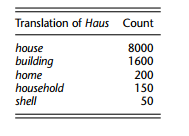
\includegraphics[scale=0.6]{Images/table1}
        \caption{Sample count data}
        \label{fig:count}
\end{figure}
Fig \ref{fig:count} shows count of translation of the word \textit{Haus} in English from \cite{koehn}.\\
Also Eq \ref{eq:3.3} represents the calculated lexical probability of translating the \textit{German} word \textit{Haus} to the following English word. \\

\begin{equation} \label{eq:3.3}
    X=
    \begin{cases}
      0.8, & \text{if e=house}\ \\
      0.16, & \text{if e=building}\ \\
      0.02, & \text{if e=home}\ \\
      0.015, & \text{if e=household}\ \\
      0.005, & \text{if e=shell}\ \\
    \end{cases}
\end{equation}
    
We can apply the above maximum likelihood hypothesis by translating for each foreign word, the English word for which the probability function is maximum. This type of translating a sentence word-by-word is very intuitive but is only useful when languages belong to same family. Because, languages of same families tend to have the same word order which is rarely the case since we always want translation between any pair of languages. Translation between any pair of languages incurs Alignment, which is mentioned in the next section.

\section{Alignment}
A pair of sentence can have the following alignment settings\cite{bhattacharyya}:\\
\begin{enumerate}
\item The source and target language are same family languages that the order of word is entirely same. 
\item The source and target language are not of same family but the sentence follows a pattern that each word from source sentence maps to only 1 word in the target language.
\item A word maps to nothing on the target sentence, i.e. null alignment.
\item Multiple words maps to same word in target sentence.
\item One word maps to multiple word in target sentence.
\item Multiple words map to multiple word in target sentence.
\end{enumerate}

\section{Factors Influencing $P(f\mid e)$}
The translation model probability, $P(f \mid e)$ is dependent on following factors:

\subsection{Alignment factor a}	
The translation probability can be expanded to included Alignmnet factor as
\begin{equation}
P(f\mid e) = \sum_{a}P(f\mid e)
\end{equation}
where a runs parallel to a. For ex Fig\ref{fig:alignment}\cite{bhattacharyya} shows a sample alignment between a e $\leftrightarrow$ f pair. Table\ref{tab:alignment} shows the equivalent alignment vector a for the sample sentence.

\begin{figure}
        \centering
        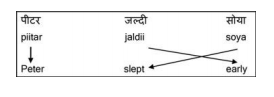
\includegraphics[scale=0.6]{Images/alignment}
        \caption{Alignment between an example e $\leftrightarrow$ f pair.}
        \label{fig:alignment}
\end{figure}



\begin{table}[h!]
\centering
 \caption{Sample alignment} 
 \label{tab:alignment} 
 \begin{tabular}{c c c c} 
 \hline
 Index & 1 & 2 & 3 \\  
 \hline
 F & Piitar & jaldi & soya \\
 a & 1 & 3 & 2 \\ [1ex] 
 \hline
 \end{tabular}
\end{table}

\subsection{Length factor \textit{m}}
Length is also another important criteria for translating sentence. It is used to control or restrict the output. Imagine a translation of a 8-word sentence to be of just 3-words or 20-words. SMT takes this factor into consideration by marginalizing the above \eqref{eq:3.3} with length(m), which becomes:
\begin{equation}
P(f,a\mid e) = \sum_{m}P(f,a,m\mid e)
\end{equation}

Combining the above two factors as together, the translation model becomes\cite{bhattacharyya}


\begin{align*}
P(f,a,m\mid e) &= P(m\mid e)P(f,a\mid e,m) \\
			   &= P(m\mid e)P(f_{1},a_{1},f_{2},a_{2},\ldots,f_{m},a_{m}\mid e,m) \\
               &= P(m\mid e)\prod_{j=1}^{m}P(f_{j},a_{j}\mid f_{1}^{j-1},a_{1}^{j-1},e,m) \\
               &= P(m\mid e)\prod_{j=1}^{m}P(a_{j}\mid f_{1}^{j-1},a_{1}^{j-1},e,m)\prod_{j=1}^{m}P(f_{j}\mid f_{1}^{j-1},a_{1}^{j},e,m) \\ 
\end{align*}
where \\
\begin{itemize}
\item Part1: Length Probability: $P(m\mid e)$ 
\item Part2: Alignment Probability: $\prod_{j=1}^{m}P(a_{j}\mid f_{1}^{j-1},a_{1}^{j-1},e,m)$
\item Part3: Translational Probability: $\prod_{j=1}^{m}P(f_{j}\mid f_{1}^{j-1},a_{1}^{j},e,m)$
\end{itemize}

So, the final Translation model becomes:
\begin{equation}
P(f\mid e) = P(m\mid e)\sum_{a}\Bigg[ \prod_{j=1}^{m}P(a_{j}\mid f_{1}^{j-1},a_{1}^{j-1},e,m)\prod_{j=1}^{m}P(f_{j}\mid f_{1}^{j-1},a_{1}^{j},e,m)\Bigg] 
\end{equation}
the three parts of equation simply means
\begin{enumerate}
\item What is the probability that $e$ generates a sentence $f$ of length m?
\item What is the probability that translation of $j^{th}$ word $f_{j}$ in $f$ would find it's alignment at position $a_{j}$ in $e$?
\item What is the probability that e's translation is $f_{j}$?
\end{enumerate}







